\documentclass[12pt]{article}
\usepackage[utf8]{inputenc}
\usepackage[T1]{fontenc}
\usepackage[brazil]{babel}
\usepackage{indentfirst}
\usepackage{multicol}
\usepackage{graphicx}
\usepackage{multirow}
\usepackage[a4paper, top = 2.5cm, bottom = 2.5cm, footskip = 1cm]{geometry}
\usepackage{vwcol}
\usepackage{subfigure}
\usepackage{url}
\renewcommand{\familydefault}{\sfdefault}

% necessário para ter várias seções dentro de seções
\setcounter{secnumdepth}{5}
\setcounter{tocdepth}{5}

\title{Manual do Bixo 2020}
\author{Centro Acadêmico Pata do Bisão, Gestão 2020}
\date{\today}

\begin{document}

%%% CAPA %%%
\begin{figure}[p]
  \thispagestyle{empty}
  \hspace*{-2.4cm}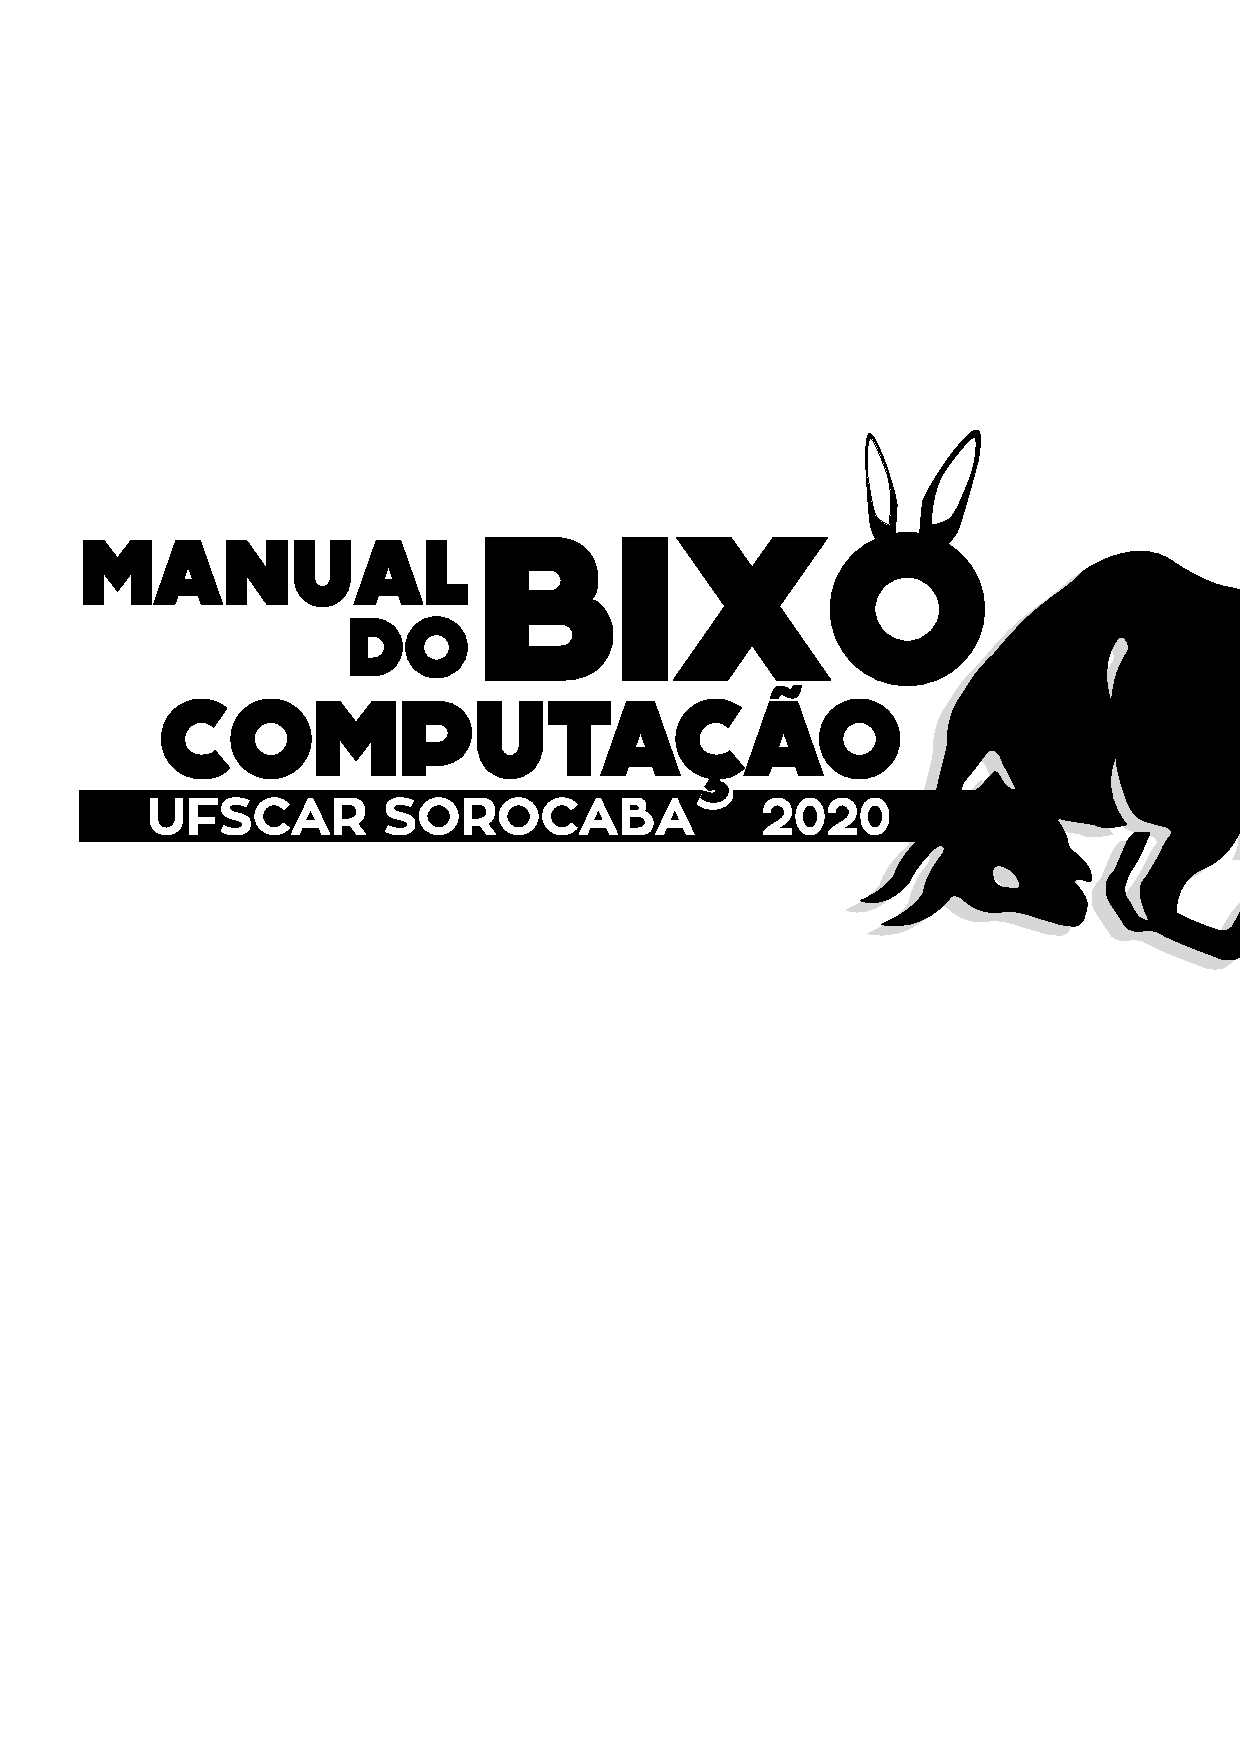
\includegraphics{./imagem/capa2020.pdf}
\end{figure}

\clearpage
\begin{center}
  Este projeto está licenciado em Attribution-ShareAlike 4.0 International da Creative Commons. Para saber mais sobre a licença, você pode visitar este website: \texttt{https://creativecommons.org/licenses/by-sa/4.0/}
~\\[\baselineskip]
  \begin{figure}[h]
    \centering
    \begin{subfigure}
      \centering
      \includegraphics[width=0.2\textwidth]{./imagem/cc_logo.pdf}
    \end{subfigure}
    \begin{subfigure}
      \centering
      \includegraphics[width=0.2\textwidth]{./imagem/by_sa.pdf}
    \end{subfigure}
  \end{figure}
~\\[\baselineskip]

  O código fonte deste manual se encontra no repositório do Centro Acadêmico Pata do Bisão, você pode visitar neste website: \url{https://github.com/caccs/Manual-do-Bixo}.


  \vfill Copyright © 2013-\the\year \thinspace Centro Acadêmico Pata do Bisão
\end{center}

\thispagestyle{empty}

\clearpage
\setcounter{page}{1}

%%% ÍNDICE %%%
\clearpage
\tableofcontents

%%% SOBRE %%%
\clearpage
\section{SOBRE ESTE MANUAL}
Este manual foi baseado em um manual dos bixos existente do Centro Acadêmico de 2013, sendo ele aprimorado e revisado desde a gestão de 2015/2 do Centro Acadêmico Pata do Bisão.

Esperamos que este manual te ajude de alguma forma sua nova vida acadêmica, calouro(a); caso você acredite que faltou algum item ou necessita de mais detalhes sobre determinado assunto, procure nossa página no Facebook e conte para gente. :)

Caso precise urgentemente de alguma informação que não esteja aqui, pode nos contactar pela página do Facebook: \texttt{https://www.facebook.com/CACCS.UFSCar/}

Por fim, gostaríamos de agradecer ao Departamento de Computação por incentivar o Centro Acadêmico em todas as atividades que propomos, incluindo o Manual do Bixo. Vocês são 10/10. <3

\begin{flushright}
  Obrigado(a)!

  C.A. Pata do Bisão Gestão 2020
\end{flushright}


%%% BEM-VINDO %%%
\clearpage
\section{GLOSSÁRIO}
\begin{itemize}
  \item \textbf{BCC:} Se alguém já te perguntou se você era da “BCC” e você ficou sem entender, aqui vai uma ajudinha: se você está matriculado em ciência da computação, você é um BCC também! (Bacharelado em Ciência da Computação).
  \item \textbf{DCE: } Diretório Central dos Estudantes, é a entidade que representa todos os discentes da UFSCar, dos quatros campi. Tendo integrantes de diversos cursos envolvidos, é a autoridade máxima dos alunos no campus, possuindo assim a responsabilidade de lutar junto à reitoria da UFSCar e à diretoria do campus Sorocaba por melhores condições de ensino.
  \item \textbf{DiGRA: }DiGRA é a sigla para Divisão de Gestão e Registro Acadêmico. Fazendo uma comparação com os tempos de ensino base, a DiGRA é como se fosse a secretaria geral da universidade.
  \item \textbf{DComp: }O DCOMP é o Departamento de Computação do nosso campus, ou seja o seu departamento. \newline Para maiores informações segue o link: \url{http://www.dcomp.sorocaba.ufscar.br/}
\end{itemize}


%%% BREVE INTRODUÇÃO AO CURSO %%%
\section{BREVE INTRODUÇÃO AO CURSO}
Independente de sua cidade natal, de estar morando sozinho, com os pais ou até em uma república, nós sabemos o quão diferente é a vida acadêmica do colégio e do cursinho. Sempre é uma grande mudança e um grande passo para qualquer jovem. Aqui nós damos algumas dicas sobre as matérias dos seus primeiros semestres e como funciona o sistema de requisitos de nosso curso.

Na UFSCar utilizamos o sistema de créditos - você pode entender créditos como horas semanais de um semestre - em que, no curso Ciência da Computação você precisará de 217 créditos para se formar sendo eles: 109 de disciplinas obrigatórias, 56 de optativas, 24 do Trabalho de Graduação ou Estágio, 22 créditos de atividades de extensão e 6 créditos de atividades complementares. Como aluno, é necessário que você complete pelo menos 8 créditos em um ciclo de um ano (contabilizando o semestre atual com o semestre anterior). Caso esse número de créditos não seja atingido, o estudante é considerado ``jubilado'' e sua matrícula é cancelada, perdendo a vaga. Além deste requisito, o calouro tem que passar em pelo menos 4 créditos no primeiro semestre para não perder a vaga. Isso pode ser reversível com a utilização do recurso (e é claro, uma justificativa convincente). Por isso muito cuidado!

O IRA (Índice de Rendimento Acadêmico) é adotado para classificação na concorrência de prioridade de inscrição de disciplinas, transferências internas e bolsas para iniciação científica.

No link abaixo temos um ilustrativo de como serão os semestres dos ingressantes.As setas representam quais matérias precisam ter aprovações para se cursar as outras.

\texttt{<https://document.li/HXB9>}

O que acontece se você por acaso não passar em uma matéria? Ele fica com a
famosa dependência ou DP, tendo de refazê-la em um semestre futuro. Note a
importância de Introdução à Programação, por exemplo, cuja DP não permite
cursar duas matérias no segundo semestre e consequentemente três matérias no terceiro, o que acaba atrasando um pouco o curso.

Brotip: Tente dar prioridade as matérias da área de matemática (Geometria Analítica e Algébra Linear, Cálculo Diferencial e Integral I) pois são matérias fornecidas pelo DFQM (Departamento de Física, Química e Matemática)
e dificilmente existem turmas extras pelo número limitado de professores, o que acaba dificultando para refazê-las.


%%% VIDA ACADÊMICA %%%
\section{VIDA ACADÊMICA}
\subsection{Sobrevivendo em Sorocaba}
Nesta seção colocaremos algumas informações importantes para que você sobreviva da melhor maneira na cidade de Sorocaba; não se deixe levar pelo título dessa seção! Viver em Sorocaba não é uma coisa do outro mundo, mas algumas informações prévias facilitarão muito sua vida.

\subsubsection{Onde Morar}
Se você, como muitos outros estudantes da universidade, não é da cidade de Sorocaba e ainda não conseguiu um lugar para morar, você pode pesquisar algo no grupo de repúblicas do Facebook <\texttt{fb.com/groups/208040842611873/}>. Lá muitos veteranos divulgam vagas em suas repúblicas.

Caso você esteja à procura de uma casa para alugar sozinho ou com amigos, segue alguns links de imobiliárias em Sorocaba:

\begin{itemize}
  \item BIS <http://www.bissorocaba.com.br/>
  \item Emaximóvel <http://www.imobiliariaemaximovel.com.br/>
  \item M\&C imóveis <http://www.imobiliariaemsorocaba.com.br/>
  \item Mendes Ortega <http://www.mendesortega.com.br/>
  \item Ribera <http://www.riberaimoveis.com.br/>
  \item Reis imóveis <http://www.reisimoveis.com.br>
  \item Casabranca Imoveis <http://www.casabrancanet.com.br>
\end{itemize}

Abaixo indicaremos lugares onde há grande quantidade de alunos da UFSCar, não
necessariamente do curso de Computação. Como são apenas endereços, você deve
procurar a portaria de cada lugar e perguntar a forma de alugar (sendo ela por
imobiliária ou direto com o proprietário), são eles:

\begin{itemize}
  \item Vila Universitária
    \begin{itemize}
      \item Travessa direita da Rodovia João Leme dos Santos (depois da UFSCar)
      \item Condomínio de chalés. Lugar bem próximo da UFSCar (especificamente 10 minutos a pé).
          Na região, não há muitas opções de mercado e também não há circular de domingo, portanto se programe.
            É um bom lugar para ter várias horas de sono e maximizar a economia do dinheiro. O preço varia de R\$600 a R\$800 (depende do proprietário/imobiliária e localização), com o condomínio incluso na grande maioria dos casos, mas você pode dividir o espaço com cerca de 3 pessoas.
    \end{itemize}

  \item Vila Universitária II
    \begin{itemize}
      \item Travessa direita da Rodovia João Leme dos Santos (depois da UFSCar)
      \item O Condomínio Universitário Vila II é composto por apartamentos de 35 m2 (metros quadrados). Localiza-se nas proximidades da UFSCar (aproximadamente 15 minutos, a pé). Recomendado para aqueles que gostam de acordar um pouco mais tarde (isso não significa que você não vai perder a hora). As despesas com o aluguel giram em torno de R\$650, onde já é incluso água, luz, gás e internet (sendo esse último item compartilhado com todos que moram, logo é um pouco lento). É possível dividir o
          local com mais uma pessoa para aqueles que querem economizar uma grana. No mais, tem uma "salinha de estudos"  (onde jogamos baralho) e uma churrasqueira.
    \end{itemize}

  \item Jambalaia
    \begin{itemize}
      \item Estrada Dr. Celso Charuri, 307
      \item Condomínio de kitnets. Lugar também bem próximo da UFSCar, não tão perto quanto a Vila Universitária, tem os mesmos contra e os pŕos da Vila. Existem três tipos de apartamento, com três preços variados. O primeiro tipo, é a kitnet. O preço varia algo entre R\$500,00 e R\$600,00, mas é impossível dividir com mais alguém. O segundo tipo, é um apartamento de um quarto. Dá pra dividir com uma pessoa e o preço fica entre R\$600,00 e R\$700,00. O último é o apartamento com dois quartos, cujo preço é algo entre R\$700,00 e R\$800. No condomínio tem uma academia, então não ficar MOnSTRO não é desculpa.
    \end{itemize}

  \item Saragoza (condomínio fechado)
    \begin{itemize}
      \item Av. Dr. Armando Pannunzio, 1791-1965
      \item{O lugar fica no final da Av. Armando Pannunzio, próximo de um ponto de ônibus que demora cerca de 20 minutos até a UFSCar, portanto fique atento aos horários do ônibus através do aplicativo da URBES. O bairro contém um McDonalds, mercados e uma galeria onde é possível encontrar pizzaria, açaí, lojas de eletrônicos, padaria e até um banco da CAIXA.
	      O aluguel é em torno de R\$800,00 para o apartamento com dois quartos, R\$1100,00 o apartamento com três quartos e R\$1300,00 a cobertura (três quartos e dois banheiros); R\$290,00 de condomínio, que inclui a conta de água. Há também um espaço de lazer que tem uma quadra e uma área para churrasco}
    \end{itemize}

  \item Portal dos Bandeirantes (condomínio fechado)
    \begin{itemize}
      \item R. Benedito Venceslau Mendes, 171
      \item O lugar fica no final da Av. Armando Pannunzio, tendo as mesmas características do Saragoza (perto do ponto de ônibus, McDonalds, mercado, etc) O aluguel é por volta de R\$800, sendo R\$200 de condomínio. O espaço de lazer tem como área para churrasco, piscina, quadra, área verde.
    \end{itemize}

  \item Mangueiras (condomínio fechado)
    \begin{itemize}
      \item Rua Orlando Bismara, 130
      \item A descrição do arredores é parecida com do Portal e do Saragoza. No espaço há uma quadra, área para churrasco, área verde com parque para crianças e um ponto de ônibus no mesmo quarteirão do condomínio. O aluguel fica em torno de R\$1200 para todos os apartamentos, sendo que eles têm três quartos --um pequeno, um grande e uma suíte-- e dois banheiros. O condomínio custa R\$270,00.
    \end{itemize}
\end{itemize}

Como última opção, existe a moradia da UFSCar. Os detalhes estão descritos na página \pageref{moradia}

Brotip: Independente do local que você escolha morar, procure conhecer melhor o bairro! A sua segurança e integridade física é mais importante do que um local mais barato.

\subsection{Transporte}
\subsubsection{Indo ou Voltando da Universidade}
Existe uma linha de ônibus em Sorocaba que tem ponto final dentro do nosso campus. O nome da linha é “UFSCAR” e o número é 80. Seu ponto de partida é o terminal São Paulo.

Os ônibus da cidade de Sorocaba não possuem cobradores. Para utilizar o transporte é preciso possuir passe, que atualmente custa R\$ 4,20 (passe social). Estudantes podem adquirir passe de ônibus por R\$ 2,00 (os ônibus da cidade tem um sistema de cartões de passes que precisam ser feitos junto a faculdade/secretária).

Brotip: A Urbes tem um aplicativo com os horários de todos os ônibus que rodam por Sorocaba. É uma boa ter pra não ficar perdendo tempo no ponto quando o próximo ônibus passa só uma hora mais tarde. É válido lembrar também que esse aplicativo pode demorar para ter seus horários atualizados (quando a faculdade entra de férias e as linhas diminuem), então fique esperto!

Para saber mais informações sobre a linha de ônibus da UFSCar acesse o link \newline{<https://www.urbes.com.br/comunidade/consulta-por-horarios>}

Para utilizar o passe de estudante, você deve registrar no site da URBES através do link <https://www.urbes.com.br/Estudantes/>

Outro detalhe importante que deve-se destacar é a possibilidade de integração entre os ônibus de Sorocaba. Isso significa que você não precisaria pagar duas viagens entre dois diferentes ônibus. (UFSCar e 9 de Julho, por exemplo). O tempo máximo da integração fica em: o tempo da viagem do ônibus + 1 hora contando a partir do ínicio da viagem ou então 3 integrações.

No caso da linha UFSCar, o tempo máximo para integração é de 1 h e 40 min e você pode observar as linhas que estão integradas neste link: \newline{<https://www.urbes.com.br/integracao-entre-linhas>}

Uma linha alternativa de ônibus que funciona todos os dias e que passa em frente ao campus (fique atento ao ponto de descida caso decisa usá-lo) é o Salto de Pirapora-Sorocaba \newline{<http://saltoemuitomais.blogspot.com.br/p/horario-de-onibus.html>}.

\noindent{Este ônibus possui cobrador e o valor atual da passagem é R\$ 5,05.}

Brotip: Para aqueles que moram nas repúblicas próximas a faculdade (Vila Universitária, Residencial Flora, Jambalaia, etc), é possível fazer a carteirinha do Piracema e, como consequência, conseguir pagar meia passagem ou até ter o passe livre. Para o passe livre é necessária a comprovação de renda. Mais informações sobre os passes de ônibus podem ser dadas na DiGRa.

\textbf{LEMBRE-SE QUE}: A linha da UFSCar não roda aos domingos e feriados! Então se você decidir morar perto da universidade e quiser passear, vai ter que usar o Piracema. Os passes de estudante do Piracema também não são aceitos aos domingos e feriados, ou seja, você tem que pagar o valor integral.

Brotip 2: Agora tem Uber em Sorocaba. Pra ir ou voltar do rolê é uma boa pedida.

\subsubsection{Voltando para Casa}
A gente sabe que os ônibus tão cada vez mais caros e, pra dar um jeito, foram
criados alguns grupos de carona no Facebook. O mais geral é esse:
\newline{<https://goo.gl/mSpWNA>}.

Nesse grupo, é possível oferecer caronas, diminuindo seus gastos e ainda ganhando uma companhia, ou procurar caronas, e aí cê vai trocando uma ideia e ainda paga mais barato.

Para algumas cidades maiores, como São Paulo e Campinas, existem grupos específicos de carona no Facebook, basta dar uma procurada no que for mais conveniente pra você.

Se, de jeito nenhum, você achar uma carona e tiver que ir para a rodoviária, fica em paz: existem ônibus que vão direto para a rodoviária saindo de ambos os terminais (São Paulo e Santo Antônio). Além disso, se você morar nas proximidades da faculdade, não precisa ir até o terminal: o UFSCAR passa em frente também. (:

%%% COMIDA %%%
\begin{multicols}{2}
  [
  \subsection{Comida}
  Embora a comida do RU seja maravilhosa e a gente coma ela todo dia, duas vezes ao dia, cinco dias por semana, às vezes enjoa, né. Por isso segue uma lista de alguns lugares que você poderia ir comer, ou então, pedir para entregar:
  ]

  \begin{itemize}
    \item \textbf{Neri Lanches}
      \newline Av. Dr. Armando Pannunzio, 1077, Vila Espírito Santo, Sorocaba - SP
      \newline \texttt{www.nerilanches.com.br}
      \newline (15) 3222-8136
  \end{itemize}
  \begin{itemize}
    \item \textbf{Habibs}
      \newline Praça Oxford (Av. Dr. Armando Pannunzio), 26, Jardim Europa, Sorocaba - SP
      \newline (15) 3003-2828
  \end{itemize}
  \begin{itemize}
    \item \textbf{Disk Salgados (entregas em Salto de Pirapora e perto da UFSCar)}
      \newline Atendimento das 15h às 22h
      \newline(15) 9 9710-3090 ou (15) 9 9134-1169
  \end{itemize}
  \begin{itemize}
    \item \textbf{Cantinho da Gê} (marmitex e restaurante)
      \newline Av. Gal. Carneiro, 706 - Vila Lucy, Sorocaba - SP
      \newline (15) 3202-4389
  \end{itemize}
  \begin{itemize}
    \item \textbf{Esfiharia e Pizzaria Canalle (entregas somente perto da UFSCar)}
      \newline Rua Ovideo Leme dos Santos, 326 - Centro - Salto de Pirapora
      \newline \texttt{www.pizzariacanalle.com.br}
      \newline (15) 3492-3700/(15) 3292-3990
  \end{itemize}
  \begin{itemize}
    \item \textbf{Seu Batata}
      \newline Rua Aparecida, 754, Jardim Santa Rosália
      \newline \texttt{www.seubatata.com.br}
      \newline (15) 3031-3233
  \end{itemize}
  \begin{itemize}
    \item \textbf{Pizzaria Bortolotto}
      \newline Rua Padre ângelo Sofia, 170, Jardim Paulistano
      \newline \texttt{www.pizzariabortolotto.com.br}
      \newline (15) 3492-2239/(15) 3292-2108
  \end{itemize}
  \begin{itemize}
    \item \textbf{Cheff Refeições e Pizzaria}
      \newline Disk marmita barato disponível no iFood.
      \newline Rua João Martins Fogaça, 289, Jardim Piazza Di Roma II
      \newline \texttt{www.cheffrefeicoeserestaurante.com.br}
      \newline (15) 3318-3572/(15) 99798-2040
  \end{itemize}
\end{multicols}

%%% DIVERSÃO %%%
\subsection{Diversão}
Para aqueles momentos nos quais você não vai aguentar mais estudar ou olhar pra tela do seu computador, deixamos aqui alguns lugares pra você bater perna e fazer algo diferente pelo menos uma vez no semestre (ou várias vezes, your call).

\begin{multicols}{2}
  [
  \subsubsection{Parques}
  ]
  \begin{itemize}
    \item \textbf{Parque das Águas}
      \newline Av. Dom Aguirre, S/N - Jardim Abaete, Sorocaba - SP
  \end{itemize}
  \begin{itemize}
    \item \textbf{Zoológico Municipal Quinzinhos de Barros}
      \newline R. Teodoro Kaisel, 883 - Vila Hortência, Sorocaba - SP
      \newline (15) 3227-5454
      \newline Ter-Dom das 9h às 17h
  \end{itemize}
  \begin{itemize}
    \item \textbf{Parque dos Espanhois}
      \newline R. Dr. Campos Sales, S/N - Vila Assis, Sorocaba - SP
  \end{itemize}
  \begin{itemize}
    \item \textbf{Parque Natural Municipal da Biquinha}
      \newline Av. Comendador Pereira Inácio, 1112 - Jardim Vergueiro, Sorocaba - SP
      \newline (15) 3224-1997
      \newline Todos os dias das 8h às 17h
  \end{itemize}
  \begin{itemize}
    \item \textbf{Prefeitura Municipal de Sorocaba}
      \newline Av. Eng. Carlos Reinaldo Mendes, 3041 - Alto da Boa Vista, Sorocaba - SP
      \newline \textit{Perfeito para caçar Pokemóns aos finais de semana}
  \end{itemize}
\end{multicols}


\begin{multicols}{2}
  [
  \subsubsection{Shoppings}
  ]
  \begin{itemize}
    \item \textbf{Shopping Iguatemi Esplanada}
      \newline Av. Prof. Izoraida Marques Peres, 401 - Campolim, Sorocaba - SP
      \newline Horário: 10h às 22h
      \newline (15) 3219-9900
  \end{itemize}
  \begin{itemize}
    \item \textbf{Shopping Cidade}
      \newline Av. Itavuvu, 3373 - Jardim Santa Cecília, Sorocaba - SP
      \newline Horário: 10h às 22h
      \newline (15) 3333-0200
  \end{itemize}
  \begin{itemize}
    \item \textbf{Pátio Ciane Shopping}
      \newline Av. Dr. Afonso vergueiro, 823 - Centro, Sorocaba - SP
      \newline Horário: 10h às 22h
      \newline (15) 3333-3333
  \end{itemize}
  \begin{itemize}
    \item \textbf{Sorocaba Shopping}
      \newline Av. Dr. Afonso vergueiro, 1700 - Centro, Sorocaba - SP
      \newline Horário: 10h às 22h
      \newline (15) 3232-2757
  \end{itemize}
\end{multicols}

\begin{multicols}{2}
  [
  \subsubsection{Bares}
  ]
  \begin{itemize}
    \item \textbf{Video Game Rock Bar}
      \newline R. Aparecida, 675 - Jardim Santa Rosália, Sorocaba - SP
      \newline Horário: Ter-Qua: 18 às 23h Sex-Sab: 18h às 2h
      \newline (15) 3442-8101
  \end{itemize}
  \begin{itemize}
    \item \textbf{Butiquim da Carne}
      \newline Av. Barão de Tatuí, 98 - Vergueiro, Sorocaba - SP
      \newline (15) 99655-9846
  \end{itemize}
  \begin{itemize}
    \item \textbf{Red Bar}
      \newline Avenida General Osório, 112 - Vila Trujillo
      \newline Horário: Ter-Qui: 17h às 1:30h
      \newline Sex-Sab: 17h às 4h
      \newline Domingo: 17 às 3h
      \newline (15) 3229-8851
  \end{itemize}
  \begin{itemize}
    \item \textbf{Retroid}
      \newline Rua Rio Grande do Sul, 420, Sorocaba - SP
      \newline Horário: 18h às 6h
      \newline Sábado: 11h às 23h Domingo: 11h às 17h
      \newline (15) 3326-6501
  \end{itemize}
  \begin{itemize}
    \item \textbf{Bar do Alemão}
      \newline Av. Eugênio Salerno, 396 - Centro, Sorocaba - SP
      \newline Horário: Ter-Sex: 11h às 15h e 18h às 23h
      \newline Sábado: 11h às 23h Domingo: 11h às 17h
      \newline (15) 3229-9111
  \end{itemize}
  \begin{itemize}
    \item \textbf{The Crown English Pub}
      \newline R. Profa. Francisca de Queiroz, 105 - Vila Indpedência, Sorocaba - SP
      \newline Horário: Seg-qui: 17h às 0h
      \newline (15) 3202-8323
  \end{itemize}
  \begin{itemize}
    \item \textbf{Hangar 51}
      \newline R. Victorio Pegoretti, 51 - Jardim Faculdade, Sorocaba - SP
      \newline Horário: Qua-Sex: 18h às 2h
      \newline Sábado: 11h às 2h
      \newline (15) 3229-8851
  \end{itemize}
\end{multicols}
\begin{multicols}{2}
  [
  \subsubsection{Lazer e Cultura}
  ]
  \begin{itemize}
    \item \textbf{Biblioteca Municipal de Sorocaba}
      \newline R. Ministro Coqueijo Costa, 180 - Alto da Boa Vista, Sorocaba - SP
      \newline Horário: Seg-Sex: 8h às 16:50
      \newline Sábado: 13h às 16:50
      \newline (15) 3228-1955
  \end{itemize}
  \begin{itemize}
    \item \textbf{Museu de Arte Contemporânea}
      \newline Av. Dr. Afonso Vergueiro, 280 - Centro, Sorocaba - SP
      \newline Horário: Seg-Sex: 9h às 17h
      \newline (15) 3233-1692
  \end{itemize}
  \begin{itemize}
    \item \textbf{FUNDEC Sorocaba}
      \newline R. Brig. Tobias, 73 - Centro, Sorocaba - SP
      \newline Horário: Seg-Sex: 8h às 18h
      \newline Sábado: 8h às 12h
      \newline (15) 3233-2200
  \end{itemize}
  \begin{itemize}
    \item \textbf{SESC Sorocaba}
      \newline R. Barão de Piratining, 555 - Jardim Faculdade, Sorocaba - SP
      \newline Horário: Ter-Sex: 9h às 21:30
      \newline Sab-Dom: 10h às 18:30
      \newline (15) 3332-9933
  \end{itemize}
  \begin{itemize}
    \item \textbf{Jardim Botânico de Sorocaba}
      \newline R. Miguel Montoro Lozano - Jardim Iguatemi, Sorocaba - SP
      \newline Horário: Ter-Dom: 9h às 17h
      \newline (15) 3227-9996
  \end{itemize}
\end{multicols}

Tem mais informações no link a seguir. Desde bares até os shows que acontecem. Sempre tem coisa legal rolando por Sorocaba, então não custa nada entrar pra dar uma olhadinha. <http://agendasorocaba.com.br/>

\begin{multicols}{2}
  [
  \subsubsection{Postos/Hospitais}
  Nesta seção colocaremos um compilado de postos de saúde e hospitais, que porventura precise, esse tipo de informação é sempre bom saber de antemão.
  Lembrando que todos os endereços que colocamos aqui são os mais próximos da Av General Carneiro por motivos de facilidade.
  ]
  \begin{itemize}
    \item \textbf{Hospital Evangélico de Sorocaba}
      \newline Av. General Carneiro, 465
      \newline (15) 2101-6600
  \end{itemize}
  \begin{itemize}
    \item \textbf{UPH Zona Leste Sorocaba}
      \newline R. Cel. Nogueira Padilha, 2585 - Vila Hortência
      \newline (15) 3333-0100
  \end{itemize}
  \begin{itemize}
    \item \textbf{Pronto Atendimento UPH}
      \newline Av. General Carneiro, 1670
      \newline (15) 3202-2495
  \end{itemize}
  \begin{itemize}
    \item \textbf{UNIMED}
	\newline R. Antonia Dias Petri, 135 - Pq. Sta Isabel
	\newline (15) 3229-3000
	\newline www.unimedsorocaba.coop.br
  \end{itemize}
\end{multicols}

\begin{multicols}{2}
  [
  \subsubsection{Gás/Água}
    Só realmente sabemos a falta que o gás faz quando ele acaba, então pra dar uma ajuda pra vocês, deixamos aqui alguns números pra vocês não passarem por esse perrengue:
  ]
  \begin{itemize}
    \item \textbf{Disk Gás Sorogás}
      \newline R. Doutoer Américo Figuereido, 576, Jardim Simus
      \newline (15) 3221-1549
  \end{itemize}
  \begin{itemize}
    \item \textbf{Depósito de Gás e Água Jardim São Paulo}
      \newline R. Dr. Benedito Cardoso Franco, 61, Vila Espírito Santo
      \newline (15) 3221-6897
  \end{itemize}
  \begin{itemize}
    \item \textbf{Disk Água General}
      \newline Av. General Carneiro, 218
      \newline (15) 3242-7800/(15) 3011-7201
  \end{itemize}
  \begin{itemize}
    \item \textbf{Almeida Gás e Água}
      \newline Rua Encarnação, 289, Wanel Ville
      \newline (15)3221-5636/(15)3011-3103
  \end{itemize}
  \begin{itemize}
    \item \textbf{CIA Gás}
      \newline Rua Leo Migliori, 51, Jardim Wanel Ville IV
      \newline (15) 3013-3949/(15) 3217-8110
  \end{itemize}
  \begin{itemize}
    \item \textbf{Disk Água General}
      \newline Av. General Carneiro, 218
      \newline (15) 3242-7800/(15) 3011-7201
  \end{itemize}
\end{multicols}

\subsubsection{Links de compras/vendas/trocas}
  \begin{itemize}
    \item \texttt{Brechó UFSCar} \texttt{<goo.gl/Wi3kgy>}
    \item \texttt{Compra e venda móveis} \texttt{<goo.gl/Ha1zob>}
    \item \texttt{Vendas barganhas em Sorocaba}\texttt{<https://goo.gl/aTUEXR>}
    \item \texttt{Laricão UFSCar Sorocaba} \texttt{<goo.gl/DKgk4q>}
  \end{itemize}

%%% ESTRUTURA/SERVICOS DA UNVIERSIDADE %%%
\subsection{Estrutura/Serviços da Universidade}

\subsubsection{E-Mail}
Vocês calouros(a) terão um e-mail com o domínio @dcomp.sor.ufscar.br que será disponibilizado pelo nosso departamento (DComp). Com ele vocês poderão agregar qualquer serviço da universidade, seja ele o SIGA, o AVA e ainda receber e-mails de bolsas atividades e de bolsas de iniciação científica enviadas normalmente pelos nossos professores. Então é estritamente importante ver os e-mails diariamente, se você não tem esse hábito, poderá perder algumas oportunidades que serão oferecidas durante a graduação.

Além disso, com este e-mail você poderá acessar alguns produtos/serviços que algumas empresas disponibilizam para estudantes de forma gratuita, na lista abaixo temos uma pequena compilação:
\begin{itemize}
  \item \textbf{Github Educational Pack} \texttt{https://education.github.com/pack}
  \item \textbf{Amazon Web Service Educate} \texttt{https://aws.amazon.com/pt/grants/}
  \item \textbf{InteliJ IDEA} \texttt{https://www.jetbrains.com/buy/classroom/?product=idea}
\end{itemize}

Obs: Esses serviços possuem a duração de 1-2 anos, sendo necessário revalidar em alguns casos (como acontece no Github Educational Pack).

\subsubsection{Biblioteca}
\noindent Funcionamento de segunda a sexta
\begin{itemize}
  \item Expediente das 8h às 22h
  \item Emprestimo e devolução de livros das 8h às 21h45
\end{itemize}
\noindent Qualquer pessoa pode entrar e ler os livros dentro do prédio, porém para os empréstimos é necessário um cadastro na biblioteca, que é feito na própria biblioteca em um período determinado.
\newline \newline Mais informações, consulte o site da B-So:
\texttt{<http://www.sorocaba.ufscar.br/bso/>}

\subsubsection{Laboratórios}
Temos quatro laboratórios, sendo três para uso específico (LSO, LSA, LARS) e um para uso geral (LEC), sendo que todos eles estão
concentrados no ATLab (Prédio Roxo) e ficam à disposição no período diurno (8h-18h).

Fora esses, ainda há mais dois laboratórios que ficam no último andar do prédio AT2 (Prédio Vermelho).
O responsável por abrir e cuidar desses laboratórios é o nosso técnico Tiago,
porém, caso seja necessário, o Centro Acadêmico também tem a permissão de
abrir os laboratórios para estudos, portanto não hesite em entrar em contato.
O horário de serviço do Tiago é geralmente das 9h -- 17h.

\subsubsection{Restaurante Universitário (RU)}
O RU é o Restaurante Universitário que temos no nosso campus. De segunda à sexta é servido aos alunos almoço e janta. Para utilizar o RU basta comprar o ticket do RU (a venda normalmente acontece do lado de fora do ambulatório) e entregá-lo na entrada.

Funcionamento de segunda à sexta: 11h às 13h30 e 17h30 às 19h

No sábado: 11h às 13h30

Tickets vendidos de segunda à sexta: 11h às 13h e 17h30 às 19h00

Valor: R\$2,16 à alunos não bolsistas.

Quer saber sobre o cardápio do RU? Acesse o link

\texttt{<https://goo.gl/QdmKYT>}

ou baixe o app do cardápio do RU feito pela Beets Jr (disponível apenas para

Android)

\texttt{<https://goo.gl/tV94j5>}

\subsubsection{Ambulatório}
Na UFSCar Sorocaba temos o atendimento de enfermagem ambulatorial (verificação da pressão arterial, da temperatura e etc), médico e também psicológico. Para receber o atendimento de enfermagem ambulatorial basta comparecer pessoalmente e apresentar a carterinha estudantil.

Já para os outros atendimentos, você deve marcar uma consulta pessoalmente ou pelo telefone, seguem eles abaixo: \\

\bigbreak
\noindent \textbf{Médico:}
\newline Dr. LUIZ FERRAZ DE SAMPAIO NETO (ginecologista)
\newline (15) 3229-5918
\newline \texttt{lfsampaio@ufscar.br}

\begin{multicols}{2}
\noindent \textbf{Psicóloga:}
  \newline FABIANA MIDORI OIKAWA
  \newline (15) 3229-5925
  \newline \texttt{fbkawa@ufscar.br}

\noindent \textbf{Enfermeira:}
  \newline SANDRA REGINA ROCHA ARAUJO
  \newline (15) 3229-5918
  \newline \texttt{sandra@ufscar.br}

\end{multicols}

\subsubsection{Secretaria}
Cada curso da UFSCar possui uma secretaria, ela é responsável por enviar e-mails sobre estágios, avisos de professores, informações da faculdade em geral. Entregas de documentos são geralmente entregues a ela.

O horário de atendimento da Secretaria é das 11:00 às 12:00 e das 13:00 às 16:30, de segunda-feira à sexta-feira.

\bigbreak
\noindent \textbf{Nome, e-mail e telefone}
  \newline Marlene Aparecida de Castilho
  \newline (15) 3229-6176
  \newline bccs@ufscar.br; mcastilho@ufscar.br; alunosbccs@ufscar.br
  \newline Brotip: Este último é o email geral de BCC. Tome cuidado ao enviar algo para esse endereço pois será automaticamente repassado à \textbf{todos os alunos do curso}.

\subsubsection{Cantina}
Até 2017 a UFSCar possuía uma cantina fixa, porém, no meio do ano, fechou por problemas de contrato. Com a saída da cantina, alunos e não-alunos passaram a vender diferentes tipos de comidas e bebidas (incluindo comidas veganas!) dentro da faculdade.

Atualmente, na entrada do prédio roxo, encontra-se uma vendinha regular com salgados, café de diferentes sabores, bolos e docinhos gerais.

\subsubsection{Xerox}
O serviço de xerox e cópias fica localizado próximo ao prédio do RU, na área de vivência. O funcionamento acontece de segunda a sexta e o expediente é das 8h às 21h.

O e-mail para envio de arquivos para impressão é: \texttt{ufscar.xerox@gmail.com}


\subsubsection{Bolsas}
A UFSCar possui um sistema de bolsas para ajudar alunos em vulnerabilidade socioeconômica, esta é uma das formas oferecidas aos estudantes para que estes possam permanecer na universidade, afinal entrar na universidade é apenas o primeiro passo de uma longa jornada!


A página da Proace (Pró reitoria de Assuntos Comunitários e Estudantis) \newline \texttt{<https://goo.gl/skuswM>} possuem mais informações sobre as bolsas e auxílio aos estudantes.


Você aluno da computação que ficou interessado também pode procurar pela assistente social do nosso campus.

\paragraph{Moradia}\label{moradia}\mbox{} \\\\
\indent A UFSCar campus Sorocaba não possui moradia dentro da universidade, neste caso a universidade aluga casas para oferecer bolsa moradia aos alunos que precisam.

Para os bolsistas dessa modalidade, além do aluguel, a universidade também é responsável por diversos gastos como água, luz, IPTU e gás.

Para saber mais sobre esta bolsa e quem tem direito à ela acesse o link

\texttt{<https://goo.gl/BqD1kq>}

\paragraph{Alimentação}\mbox{} \\\\
\indent Os alunos que possuem bolsa alimentação têm direito à duas refeições diárias (almoço e janta) no RU gratuitamente, além de uma marmita nos sábados.

Maiores informações sobre esta bolsa podem ser encontradas no link

\texttt{<http://www.proace.ufscar.br>}


\paragraph{Atividade}\mbox{} \\\\
\indent Este é um tipo de bolsa onde o aluno desenvolve uma atividade 8 horas por semana durante oito meses (4 meses no primeiro semestre e 4 meses no segundo) e recebe uma ajuda de custo pela atividade desempenhada.


O link para se obter mais informações é:
\texttt{<https://goo.gl/Ucto9P>}

\subsection{Como Estudar}
Ao entrar na faculdade, geralmente temos a impressão de que vai ser igual ao ensino médio, ou pelo menos bastante parecido. Eis o que nós veteranos podemos afirmar com convicção: não é nem um pouco parecido. Então pra dar aquela ajuda, separamos algumas dicas de estudo que aprendemos na marra.

\subsubsection{Não deixe pra última hora}
Essa dica parece meio boba, mas a real é que a gente no começo sempre acha que vai dar tempo. Evite fazer isso. Diferente do ensino médio, o conteúdo não costuma vir mastigado e, às vezes, é necessário bastante estudo extra-classe. Portanto estude com antecedência sempre que possível (às vezes realmente não é)! Isso te ajuda em vários aspectos: você tem tempo para tirar dúvidas com o seu professor ou monitor, você pode revisar a matéria um dia antes da prova só pra conferir tudo e você tem mais chances de ter uma boa noite de sono antes da prova.

\subsubsection{Vá nas monitorias e no atendimento do professor}
O nosso curso tem bastante disciplina prática, o que significa que passamos bastante tempo programando e mais tempo ainda olhando pra tela do computador pensando em como resolver um problema que aparece. Em alguns casos, você não vai conseguir achar o erro de jeito nenhum e é pra isso que servem os atendimentos e as monitorias: ninguém melhor do que alguém que já fez a disciplina para te ajudar.

Aliás, não é somente nas disciplinas práticas que você às vezes esbarra nas dificuldades: as disciplinas teóricas também apresentam algumas surpresas. Pra nossa sorte, elas também têm atendimento dos professores e/ou monitoria!

Não tenha vergonha e vá perguntar! A gente tá aqui na faculdade pra aprender mesmo e eles tão na faculdade pra ajudar a gente e nos indicar qual o melhor caminho para resolver um problema.

\subsubsection{Faça as listas}
Essa dica parece besta e em alguns momentos simplesmente não dá tempo de fazer as listas, mas, sempre que der, faça. Para as disciplinas teóricas é um excelente modo de você aprender a colocar no papel o que você só saberia explicar falando (inclusive isso é um baita treinamento pra hora da prova). Para as disciplinas práticas, é o momento de você ver funcionando os conceitos aprendidos.

Brotip: Alguns professores baseiam provas nas listas de exercícios, portanto não fique vacilando achando que nada da lista cai porque tem conteúdo porque cai sim.

Brotip 2: Alguns professores \textbf{escolhem} uma questão da lista pra por na prova. Uma questão faz muita diferença.

\subsubsection{Fale com seus veteranos}
Procure gente que já fez a disciplina e pergunte qual a melhor forma de estudar. Cada professor tem um estilo de prova e é bem legal quando a gente não é surpreendido por um tipo de questão que não estávamos esperando. Fora isso, muitos veteranos têm uma memória ótima e podem lembrar mais ou menos do conteúdo da prova que ele fez quando cursou a disciplina.
Recomendamos a participação no grupo geral da computação no Facebook, lá estão praticamente todos os alunos e ex-alunos do curso, rolam discussões sobre as matérias, docs colaborativos e todos se ajudam com dúvidas da matéria, listas e provas. Portanto quando tiverem a oportunidade peçam para algum veterano te adicionar no grupo.

\subsubsection{Não se desespere}
Cada um tem o próprio jeito que funcionar que dá certo. Essas dicas são bem genéricas e não são lei. Tem gente que acha muito melhor estudar cinco minutos antes da prova e tem gente que com duas semanas de antecedência já está pegando o livro na biblioteca. Se nenhuma delas der certo pra você, significa que você não achou o seu jeito ainda.

Só não desanime!

No começo é difícil pra todo mundo, mas logo você pega o jeito.
\end{document}


%%% VIDA FORA DA ACADEMIA %%%
\section{VIDA FORA DA ACADEMIA}
Sim, existe vida fora da academia e não pense em ser frangão nessa parte, bixo. A universidade e os próprios alunos oferecem outros tipos de atividades pra você interagir com as pessoas do seu curso e fora também. A participação não é obrigatória, mas é sempre muito legal comparecer (e às vezes te rende uns créditos extras).

\subsection{Centro Acadêmico}
O C.A. é uma entidade estudantil constituida pelos alunos do mesmo curso e tem como objetivo levar demandas perante os conselhos que existem dentro da universidade para lutar por melhorias, seja opinando nas ementas do curso, no projeto pedagógico e também na infraestrutura da universidade. Essa entidade também é responsável por criar eventos com caráter social e produzir materias de apoio, como este próprio manual. No nosso caso, que é o curso de Ciência da Computação, a chapa eleita da gestão de 2020 é a Pata do Bisão, que nesse momento estamos conta com 10 membros ativos. Temos diversos projetos e estamos sempre querendo membros para poder ajudar neles! Se você tiver uma ideia muito bacana e/ou queira ajudar, converse conosco! Participem de nossas reuniões para que possamos cada vez melhorar nosso curso! Você pode nos contactar pela página do Facebook: \newline \url{http://www.facebook.com/CACCS.UFSCar/}

\subsection{Atlética Raça Brisão}
A atlética é uma entidade organizada por estudantes dentro das universidades. Nosso campus possui uma Atlética Geral e nosso curso também possui uma atlética, a “Atlética Raça Brisão”, responsável pela realização de eventos esportivos, culturais e sociais, dentre outras atividades.

\subsection{Semana da Computação}
A SeCoT (Semana de Computação e Tecnologia) é um evento organizado pelos alunos do curso que tem como objetivo difundir em palestras e/ou workshops, novas tecnologias, metodologias e discussões que permeiam a computação e inovação. A semana é gratuita e aberta à todas as pessoas da região. Você pode ver mais informações na página do Facebook: \newline \url{https://www.facebook.com/secot.ufscar/}

\subsection{Mini Maratona de Programação}
A Mini Maratona de Programação é o evento que encerra a SeCoT. É feita nos moldes da famosa Maratona de Programação da ACM-SBC, onde grupos de três pessoas enfrentam uma sequência de problemas desafiantes de programação.

\subsection{GameDev}
A GameDev desenvolve jogos em grupos, pesquisando e aprendendo tecnologias e ferramentas em projetos que envolvem diversos aspectos de Game Design, ou Projeto de Jogos como programação, jogabilidade, arte, música e gerenciamento de projetos. \newline
O grupo é estruturado em um grupo geral, com todos os integrantes ativos, e os grupos de trabalho, onde cada grupo desenvolve um jogo. Um membro pode pertencer a um ou mais grupos de trabalho, em qualquer área de sua preferência.

\subsection{Esportes}
A Atlética Geral oferece treinos de diversas modalidades esportivas, tais como Basquete, Futebol, Vôlei e Handball. Também ocorrem amistosos contra as outras faculdades de Sorocaba.

Dentro da UFSCar ainda há o Interbixos, que é o campeonato entre os cursos com times apenas de calouros, e o Intercursos. Ambas são ótimas oportunidades pra interagir com seus colegas de classe e de curso. A página do Facebook é: \url{https://www.facebook.com/atleticaufscarsorocaba/}

\subsection{Bateria Chapelaria}
A Bateria Chapelaria procura representar nossa universidade em eventos, tanto dentro quanto fora do ambiente universitário. Seja animando festas, jogos ou mesmo chamando a atenção para assuntos de caráter político e de interesse dos alunos em geral.

A bateria é aberta para todos, são promovidas escolinhas e oficinas para quem tem vontade de aprender a tocar algum instrumento. Segue a página do Facebook: \newline \url{https://www.facebook.com/bateriachapelaria}

\subsection{Empresa Junior Beets}
A Beets é uma empresa júnior gerida e integrada por estudantes do curso de Ciência da Computação da UFSCar - Sorocaba, a qual, contribui com o desenvolvimento de soluções de TI da região, além de propiciar aos seus membros a oportunidade de vivência e aperfeiçoamento profissional. Para mais informações, tem a página no Facebook: \newline \url{https://www.facebook.com/beetsjr/}

\subsection{Iniciação Científica (IC)}
A iniciação científica (IC) é uma atividade de pesquisa desenvolvida por alunos da graduação com o apoio de um professor orientador que seja da área em que o trabalho é realizado.

Esta atividade é uma ótima forma dos alunos terem um primeiro contato com a pesquisa científica, uma vez que a maioria dos alunos não possuem experiência e terão o apoio e acompanhamento de um orientador.

A iniciação científica pode ser feita com ou sem bolsa, tudo dependerá do seu projeto ser aprovado por uma agência financiadora,  como por exemplo CNPq (Conselho Nacional de Desenvolvimento Científico e Tecnológico) e FAPESP (Fundação de Amparo à Pesquisa do Estado de São Paulo). 

Se você tem interesse em fazer uma iniciação científica, fique atento às chamadas para interessados em IC. Nossos professores divulgam com frequência oportunidade de trabalhos para os alunos que desejam fazer pesquisa. Ou então você pode apresentar à algum professor uma ideia de trabalho que você tenha para que ele possa te orientar.

\subsection{Monitoria}
A Monitoria é uma atividade extracurricular em que o aluno se encarrega em auxiliar o professor de uma determinada matéria, sanando dúvidas dos alunos que comparecerem ao horário de atendimento e passando trabalhos extraclasses; sendo possível essa atividade ser realizada com bolsa ou voluntariamente.

Todas as monitorias valem quatro créditos, sendo 12 horas reservadas semanalmente para esta atividade.

\subsection{Share Centro de Línguas}
A entidade Share é um Centro de Línguas da UFSCar que tem como objetivo incentivar o compartilhamento de línguas, no qual os alunos aprendem idiomas através das experiências linguísticas adquiridas pelos professores. As aulas são gratuitas.
Mais informações vocês podem encontrar na página do Facebook:

\url{https://www.facebook.com/ShareLinguas/}

%%% GLOSSÁRIO %%%
\section{GLOSSÁRIO}
\begin{itemize}
  \item \textbf{BCC:} Se alguém já te perguntou se você era da “BCC” e você ficou sem entender, aqui vai uma ajudinha: se você está matriculado em ciência da computação, você é um BCC também! (Bacharelado em Ciência da Computação).
  \item \textbf{DCE: } Diretório Central dos Estudantes, é a entidade que representa todos os discentes da UFSCar, dos quatros campi. Tendo integrantes de diversos cursos envolvidos, é a autoridade máxima dos alunos no campus, possuindo assim a responsabilidade de lutar junto à reitoria da UFSCar e à diretoria do campus Sorocaba por melhores condições de ensino.
  \item \textbf{DiGRA: }DiGRA é a sigla para Divisão de Gestão e Registro Acadêmico. Fazendo uma comparação com os tempos de ensino base, a DiGRA é como se fosse a secretaria geral da universidade.
  \item \textbf{DComp: }O DCOMP é o Departamento de Computação do nosso campus, ou seja o seu departamento. \newline Para maiores informações segue o link: \url{http://www.dcomp.sorocaba.ufscar.br/}
\end{itemize}


%%% LINKS ÚTEIS %%%
\section{OUTROS LINKS ÚTEIS}
Neste link vocês poderão encontrar diversas informações úteis, tanto para o curso quanto para a vida acadêmica no geral.

\begin{itemize}
% \item Manual do bixo feito pelo departamento de curso \newline \url{http://www.dcomp.sor.ufscar.br/?page\_id=664}

\item Proace (Pró-Reitoria de Assuntos Comunitários e Estudantis) \newline \url{http://www.proace.ufscar.br}

% \item Dúvidas Frequentes \newline \url{http://www.prograd.ufscar.br/duvidas.php}

\item Projeto Pedagógico do Curso \newline \url{https://dcomp.sor.ufscar.br/wp-content/uploads/2012/07/Projeto}\newline \url{PedagogicoBCCS2017_v31_CoG-Deg-So.pdf}

\item Pós Graduação em Ciência da Computação - UFSCar Sorocaba \newline \url{http://www.ppgccs.net/}
\end{itemize}

\clearpage
%%% MAPA DA UFSCAR %%%%
\section{GLOSSÁRIO}
\begin{itemize}
  \item \textbf{BCC:} Se alguém já te perguntou se você era da “BCC” e você ficou sem entender, aqui vai uma ajudinha: se você está matriculado em ciência da computação, você é um BCC também! (Bacharelado em Ciência da Computação).
  \item \textbf{DCE: } Diretório Central dos Estudantes, é a entidade que representa todos os discentes da UFSCar, dos quatros campi. Tendo integrantes de diversos cursos envolvidos, é a autoridade máxima dos alunos no campus, possuindo assim a responsabilidade de lutar junto à reitoria da UFSCar e à diretoria do campus Sorocaba por melhores condições de ensino.
  \item \textbf{DiGRA: }DiGRA é a sigla para Divisão de Gestão e Registro Acadêmico. Fazendo uma comparação com os tempos de ensino base, a DiGRA é como se fosse a secretaria geral da universidade.
  \item \textbf{DComp: }O DCOMP é o Departamento de Computação do nosso campus, ou seja o seu departamento. \newline Para maiores informações segue o link: \url{http://www.dcomp.sorocaba.ufscar.br/}
\end{itemize}

\thispagestyle{empty}

\end{document}
